Ideas to extend the measurement of lightning conference paper.

\ed{STEF: Test locally what happens if the node terminating the channel to meaure is not active).}

\ed{STEF: see what happens with max capacity + $\epsilon$}

\section{Lightning channel capacity measurement from a measuring node}
We describe a procedure to estimate node capacities of a path in the Lightning network. 
An estimation of the capacity is expressed as a lower bound/upper bound pair, namely $\langle \lambda_{min}, \lambda_{max} \rangle$ of the capacity this node have at a given instant. 
To do so, we connect a measurement node, $N_0$, under our control, to another Lightning nodes and perform different payment attempts to probe the network capacity.

Figure~\ref{fig:measurement-topology-extended} depicts the reference topology for this measurement: 
Lets consider a path formed by channels $C_0$ (between $N_0$ and $N_1$), $C_1$ (connecting $N_1$ and $N_2$), $C_2$, etc.
We assume that we know an estimation of the capacity of channels $C_0$, $C_1$, ..., $C_{i-1}$, and we want to estimate the capacity of $C_i$, i.e., $\lambda_i$.


\begin{figure}[h!]
    \centering
    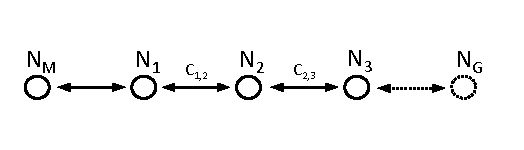
\includegraphics[width=0.95\linewidth]{img/measurement-topology-extended.pdf}
    \caption{Measurement topology extended to nodes two hops away}
    \label{fig:measurement-topology-extended}
\end{figure}


% We present EnoughCapacity
The measuring node can determine if the capacity of a channel $C_{x}$ exceeds a test value $t$ ($t<\lambda_i, \forall i < x$). 
To do so, $N_0$ performs a payment of $t$, to a \textit{ghost} node $N_G$.
This ghost node is a non-existent node, for which we generate a (non-existent) channel $C_{G}$ with a random identifier.
As the Lightning routing system is not aware of the ghost node, we 
 append to the path information provided by the routing system the information corresponding to the last hop to $N_G$.
Thus, the resulting payment request, issued with a \texttt{sendtoroute} Lightning command, has a route $C_{0} \rightarrow C_1 \rightarrow \ddots C_x, C_{G}$. 
As neither of the nodes from $N_0$ to $N_{i-1}$ validate the path with their routing information, the payment request is forwarded as long as enough capacity exits. 
However, if the request arrives to $N_i$, this node discards it, as it certainly knows there is no such channel connected to it. 
Then the transaction is aborted, and an informative a message is sent back to $N_0$.
Upon the reception of this message, we can deduce that $t \leq \lambda_{0}$, ... $t \leq \lambda_{i-1}$ and (more important to us) $t \leq \lambda_{i}$, the channel to measure.
On the other hand, if $t > \lambda_{i}$, then $N_i-1$ responds with a message indicating that there is no enough capacity, and also aborts the transference. 
In any of those cases, no hash-lock contracts are established, as they are only created from the payment receiver, in the direction to the issuer (would be created from $N_G$ to $N_i$, etc.), so no funds are blocked. 
Besides, as the computation requirements for this operation of checking and aborting are very low, the whole process is generally completed in less than a second.
We formalize the mechanism described above as a \textsc{EnoughCapacity} procedure, that takes a path, a channel to test, and a value, and returns whether the capacity at the channel is equal or higher than the test amount, or lower. 
The procedure reports an error if any of the precedent channels indicate that there is not enough capacity to make the payment progress.

We know present an algorithm to estimate $\langle \lambda_{i,min}, \lambda_{i,max} \rangle$ the capacity of channel $C_i$ in a path, assuming an estimation of the capacities of the previous channels in the path are known. 
In particular, we use the estimated capacity of the previous node, $\langle \lambda_{i,min}, \lambda_{i,max} \rangle$.
We also use $\Lambda_{i}$, the funding capacity of $C_{i}$, 
\ed{[Do this] which we obtain from matching the information of the Lightning routing system with the transactions performed into the blockchain. We have observed in some cases that the available capacity of a channel exceeds the capacity advertised by the Lightning routing system. This occurs because some nodes are configured to advertise a capacity value lower than the actual capacity commited to in the blockchain ledger.}

Apart from the lower/upper bounds for $\lambda_i$, the algorithm also indicates 
if the maximum value of the capacity is below or equal any tested capacity. 
This indicates when the capacities of the previous nodes prevented testing the maximum capacity.
We will exclude this nodes for statistics in which we count the channels having maximum capacity.

It does not aims to characterize capacities of channels that are behind others with empty (in the testing direction) capacity.


\begin{algorithm}
    \begin{algorithmic}[1]
    \Procedure{EstimateCapacity}{$\lambda_{i-1,min}$, $\lambda_{i-1,max}$, $\Lambda_{i}$, $K$}

    % Test 0 capacity, common for all cases
    % Note previous paths may have 0 capacity, or unknown (previous paths had 0 capacity)
    \If{$\lambda_{i-1, max} == 0$}
        \State return Error
        \Comment{Cannot estimate capacity if previous channel is empty}
    \EndIf

    % Test 0 capacity
    \If{! \Call{EnoughCapacity}{$C_{i}$, $\epsilon$}}
        % min, max, maximum could be tested
        \State return 0, 0, True
    \EndIf
        
    
    % We are not sure if the capacity of i is higher or equal than declared for i-1, just check
    \If{$\lambda_{i, max} \geq \Lambda_{i-1}$}
        % EnoughCapacity now has a target channel (i.e., the route stops there)

        \If {\Call{EnoughCapacity{$C_{i-1}$, $\Lambda_i$}}}
            \State $\lambda_{i-1, min}$ := $\Lambda_i$
        \EndIf
    \EndIf

    % We now know if the capacity of previous paths is  higher or not than funded for this
    \If{$\lambda_{x-1, min}  \geq \Lambda_x$ }
        % we can measure maximum values for x
        \If{\Call{EnoughCapacity}{$C_{i}$, $\Lambda_x$}}
            \If{not \Call{EnoughCapacity}{$C_{i}$, $\Lambda_i + \epsilon$}}  \Comment{Capacity is larger than advertised}
            % Maximum was tested, but result is not satisfactory
            \State return $\Lambda_i$, $\Lambda_i + \epsilon$, False
            \Else
                \State return $\Lambda_i$, $\Lambda_i$, True
            \EndIf
        \Else
            $\lambda_{i, max}$ := $\Lambda_i$
        \EndIf
    \Else
        % if i has maximum capacity, we cannot find it
        % Test if capacity is the maximum of the previous path
        \If{\Call{EnoughCapacity}{$C_{i}$, $\lambda_{i-1, min}$}}
            % This margin can be broad
            \State return $\lambda_{i-1, min}$, $\Lambda_i$, False
        \Else
            $\lambda_{i, max}$ := $\lambda_{i-1, min}$
        \EndIf
    \EndIf

    % Binary search, with proper adjusted maximum
    \State
    % lambda target for x
    \State $\lambda_{i,t}$ := $\lambda_{i, max} / 2$
    \State $\lambda_{i, min}$ := 0
    \State counter :=0    
    \While {counter $< K$}
        \If{\Call{EnoughCapacity}{$\lambda_{i,t}$}}
        \State $\lambda_{i,min}$ := $\lambda_{i,t}$
        \State $\lambda_{i,t}$ := $\frac{\lambda_{i, min} + \lambda_{i,max}}{2}$
        \Else
            \State $\lambda_{i,max}$ := $\lambda_t$
            \State $\lambda_{i,t}$ := $\frac{\lambda_{i,min} + \lambda_{i,max}}{2}$
        \EndIf
        \State counter := counter + 1
    \EndWhile 
    

    \State return $\lambda_{i,min}$, $\lambda_{i,max}$, True

    \EndProcedure
    \end{algorithmic}
    \caption{Find a lower and upper bound for  $\lambda_{x}$ in a maximum of $K+2$ iterations}
\label{alg:actual-capacity-x-hops}
\end{algorithm}


To increase the chances of a larger number of channels measured, $N_0$ connects with a capacity equal to the maximum transferable value defined by the Lightning specification, XXX. 

The algorithm presents the following properties: $\lambda_{i,min}$ is monotonically decreasing with $i$. 
However, $\lambda_{i,max}$ may increase, as it depends on the funding capacity of the channel.
We assume the error to be 0 when we match with the maximum capacity or empty channel. 
The error for a binary search is $min(\lambda_{i-1, min}, \Lambda_{i}) 2^{-(k+1)}$.
The error for the estimation of a channel $C_i$ with higher capacity than $\lambda_{i-1, min}$ is unbounded.
[Note that measures with T have a bounded error (either 0 or binary search error), while entries with F have unbounded error. When having to measures for the same channel, always prefer T over F.]

To illustrate the behavior of the algorithm, we consider the following case (for simplicity, we use small integer values for the funding and actual capacities):

\begin{table*}[]
    \begin{tabular}{llllllll}
     & $C_0$ & $C_1$ & $C_2$ & $C_3$ & $C_4$ & $C_5$ & $C_6$\\
    Maximum capacity for $C_i$, $\Lambda_i$ & 20 & 20 & 10 & 15 & 10 & 15 & 15 \\
    Current capacity for $C_i$, $\lambda_i$ & 20 & 18 & 10 & 5 & 10 & 10 & 3 \\
    $\lambda_{i, min}$ & - & 17.5 & 10 & 5 & 5 & 5 & 2.5 \\
    $\lambda_{i, max}$ & - & 20 & 10 & 6.5 & 10 & 15 & 3.125  \\
    Ensure maximum value is withing range & - & T & T & T  & F & F & T
    \end{tabular}
\end{table*}

To illustrate the behavior of the algorithm, we now execute the procedure with the channel configuration depicted in the table, and $K=3$. 
The maximum payment that can be made is 20, so this is the value for $\Lambda_0$ and $\lambda_0$.
We start with $C_1$. The test for empty capacity fails. Then, as the previous capacity is the maximum,
we can test $C_1$ for its funded capacity $\Lambda_1$, 20, which also fails.
Thus, a binary search is started within 0 and 20. Values of 10, 15, and 17.5 are tested, to generate a final bound pair of $<17.5, 20>$.

We now consider $C_2$. As $\lambda_{1,min}$, 17, is higher than $\Lambda_2$, 10, the mechanism tests the channel for its maximum capacity, which it succeeds. Therefore, the capacity estimation is $\langle 10,10 \rangle$.

For $C_3$, after testing the empty path, and being aware that the maximum capacity is 15, larger than the measured capacity for the precedent channel we start checking a value of 10. As the test indicates that the current capacity is lower, a binary search is conducted, to result in a value of $\langle 5, 6.25\rangle$. Note that even the value of 5 was specifically tested, the binary search cannot determine exact values, so a range (including the real value as a minimum) is reported.

We next process channel $C_4$. As the capacity of this channel is higher than the capacity of the previous, the algorithm responds with an estimation of $\langle 5, 10\rangle$.
For channel $C_5$, the situation is similar, with an estimation of $\langle 5, 15\rangle$

Finally, for $C_6$, when we test the minimum value of the previous channel, 5, it indicates that $\lambda_6$ is lower, so the binary search is started for the interval $\langle 0,5\rangle$, resulting in an estimation of $\langle 2.5, 3.125\rangle$.

\section{Evaluating Lightning network capacity}
Devise strategy for the measurements (to which nodes I should connect).

For measuring the channel capacity in the Lightning network, we propose the following strategy: 
We select the node with more channels of the highest funding capacity attached, according to the routing information.    
Then, we perform the process described in the previous section for channel estimation. 
We annotate the information in the routing graph. Then, we select the top node with a highest number of channels of the highest funding capacity for which no capacity estimation has been performed.
We estimate the channel capacities, annotate, and repeat the procedure until every channel has been characterized.

We first perform a 'dry run' of this scheme over the routing information data. For this case, we consider that the current capacity is equivalent to the funding capacity, although the nodes performing the measurement do not know this in advance. 
In figure [FIG] we show the number of channels characterized by this mechanism. 

[FIG] 
Draw the ccdf of the number of 
- total number of channels characterized
- number of  channels characterized as T
- number of channels characterized as F
x-axis: each round, from first to last.

We observe that... (maybe with few nodes it is enough to characterize most of the channels)
Decide with this how many rounds we may need in the real case.

We now apply the same scheme to real measures over the lightning network. 
We now observe ...

[Same figure as previous for the number of channels characterized]

At the end of the characterization process, we observe (similar to the results of the other paper...)

In addition to the results of the other paper, add these results
- number of channels that we can characterize, \% of the total number. Count high quality values (=T). Should be quite high.
- insist in matching values for the same channel observed in different measurements. Prefer T values over F. Be careful, as values may change over time, and measurements from different points (=made at different time) may measure different values.
I think that matching values support our methodology, while non-matching can be everything (this is a win-win :-))

\section{Evaluating the evolution of Lightning channels capacity over time}
[When repeating a measure (measuring a channel for which we have a previous value), we can start by checking if the previous capacity holds, with a previous +/- $\epsilon$ test.]

% We cannot select many, as it takes some time to measure.
We select randomly 1,000 channels and we observe the evolution over time of their capacities. 

Measure Lightning channel capacity one day, the day after, next week, next month, and compare the variation in the channel balance. 
This is a lower bound on the amount of money moved by Lightning (may be there are changes that we are not observing, moving in one direction, in other, etc.) 
Can be used to estimate the maturity of the network.

For this measure, we want to measure many channels in a short period of time: it the measure takes long, we may not be fast enough to measure the channels from one day to the other. Besides, a snapshot of the state is more valuable if the information of all the channels correspond to the same time. 

To be efficient in the previous task, measuring many channels in short periods of time, 
we want to connect to the lowest number possible of nodes, as establishing a channel with them takes long time 
(bitcoin transaction to create the channel, then bitcoin transaction to remove it). 
We cannot have multiple channels in parallel, as each channel requires the temporal assignment of a large amount of money. 
Besides, each time a channel is established and removed, we spent money. 

Therefore, we could formulate the problem as develop an algorithm that measures all the network by connecting to the lowest possible number of existing nodes.

